\documentclass[a4paper,11pt]{article}
\usepackage[left=2.5cm, right=2.5cm, top=1.5cm, bottom=1.5cm]{geometry}
\usepackage{graphicx}
\usepackage{amssymb}
\usepackage{amsmath}
\usepackage{hyperref}
\usepackage{cleveref}
\usepackage{float}
\usepackage[table,xcdraw]{xcolor}
\usepackage{subcaption}

\hypersetup{ %color attributes of citation, link, etc.
    colorlinks=true,
    linkcolor=blue,
    filecolor=gray,
    urlcolor=blue,
    citecolor=blue,
}

\setlength{\parindent}{0pt}

\newcommand{\matlab}{\textsc{Matlab}} %very important and totally necessary addition
\newcommand{\parallelsum}{\mathbin{\!/\mkern-5mu/\!}}

\newcommand\Item[1][]{%
  \ifx\relax#1\relax  \item \else \item[#1] \fi
  \abovedisplayskip=0pt\abovedisplayshortskip=0pt~\vspace*{-\baselineskip}}

%'codify' text for snippets
\usepackage{xcolor}
\definecolor{codegray}{gray}{1}
\newcommand{\code}[1]{\colorbox{codegray}{\texttt{#1}}}


\graphicspath{ {./images/} }
           
\begin{document}
\title{\LARGE{\textbf{ECEN405 D-Class Amplifier}}\\ \large{\textit{`What a buck converter would say if it could talk'}}}
\author{Niels Clayton : 300437590\\
\textbf{Team Members:} Daniel Eisen \& Nickolai Wolfe}
\date{}
\maketitle

\begin{center}
    \vspace{-20pt}
    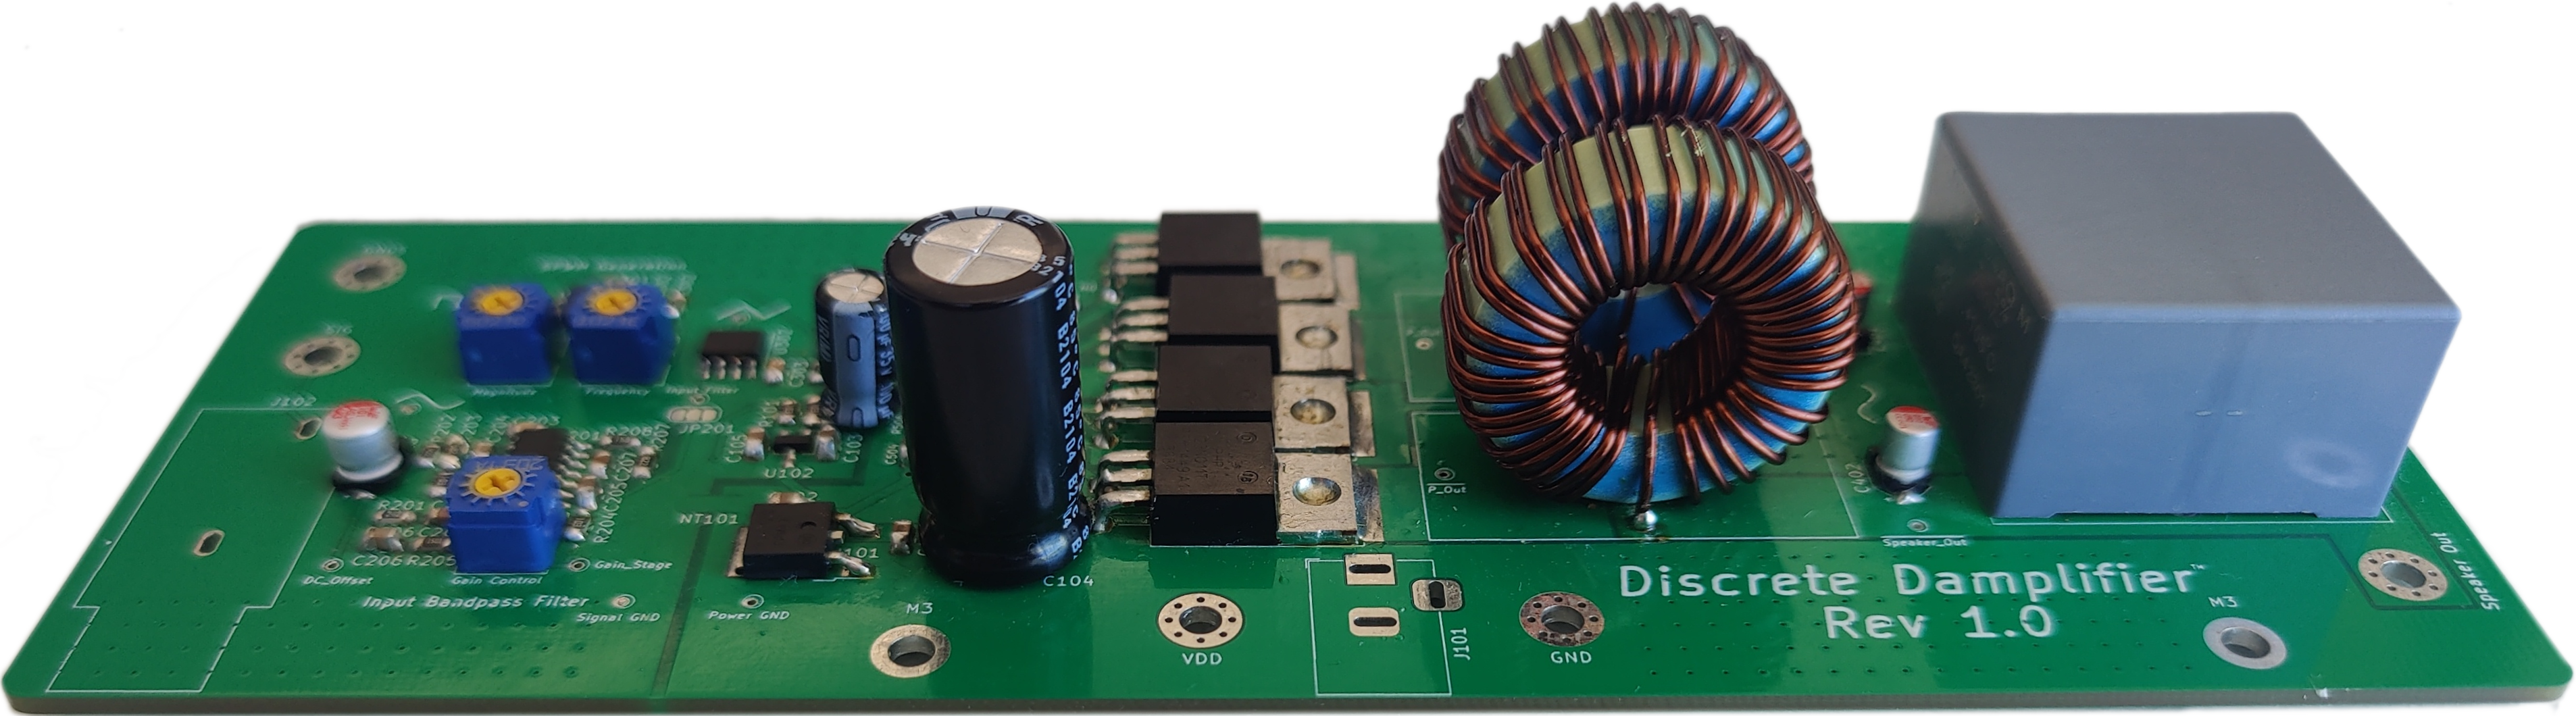
\includegraphics[width=0.9\textwidth]{design.png}
\end{center}

\section{Introduction}

Audio amplifiers facilitate the driving of high power speakers from small signal audio outputs. Common amplifier types for high fidelity audio are the class A and AB amplifier. These amplifiers provide high power outputs and very little distortion, with the limitation of low power efficiency.

In contrast, the class D amplifier is a high efficiency power amplifier with the limitation of design complexity and requiring large amounts of output filtering.\\

The operation of a class D amplifier can be broken down into discrete sections that can be seen outlined in \Cref{F:block}. From this figure we can see that the input audio signal is first filtered to remove unwanted components. This signal is then sampled at high frequency and amplified to a high power output. Finally this sampled signal is then filtered to remove the sampling frequency, providing a low distortion high efficiency output.

\begin{figure}[h!]
    \centering
    \frame{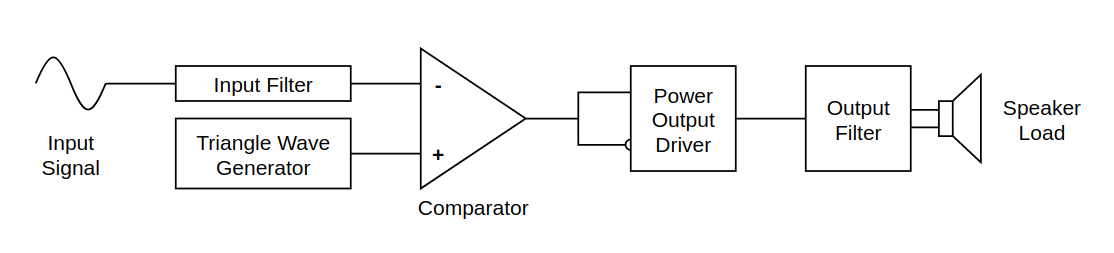
\includegraphics[width=0.8\textwidth]{block_diagram.png}}
    \caption{D-Class amplifier high level block diagram}
    \label{F:block}
\end{figure}

The purpose of this reports is to discuss the design and implementation of a class D amplifier for use in driving a sub-woofer speaker to given specifications outlined in \Cref{S:specs}. This project was completed in a group of three, where I have taken responsibility for the audio sampling and sinusoidal pulse width modulation (SPWM) generation designs. We have all contributed equally to the final PCB and schematic designs. 

\subsection{Specifications}\label{S:specs}

\begin{itemize}
    \item Supply 80W of power into a 4$\Omega$ load.
    \item Have a 10Hz to 200Hz operating bandwidth.
    \item Have an input sensitivity of 1V for maximum output.
    \item Cost a maximum of \$50 per unit.
\end{itemize}

\section{Design}

\textit{Here you should describe how your class D amplifier works, giving details of each subsection. In detail, you should describe the section you designed and the design choices you made. If your team broke up the design of the amplifier in a way that doesn’t suit individual parts being discussed, you will need to talk about the whole design in a bit more detail but you should also describe how the work was delegated and why.}

\begin{figure}[h!]
    \centering
    \frame{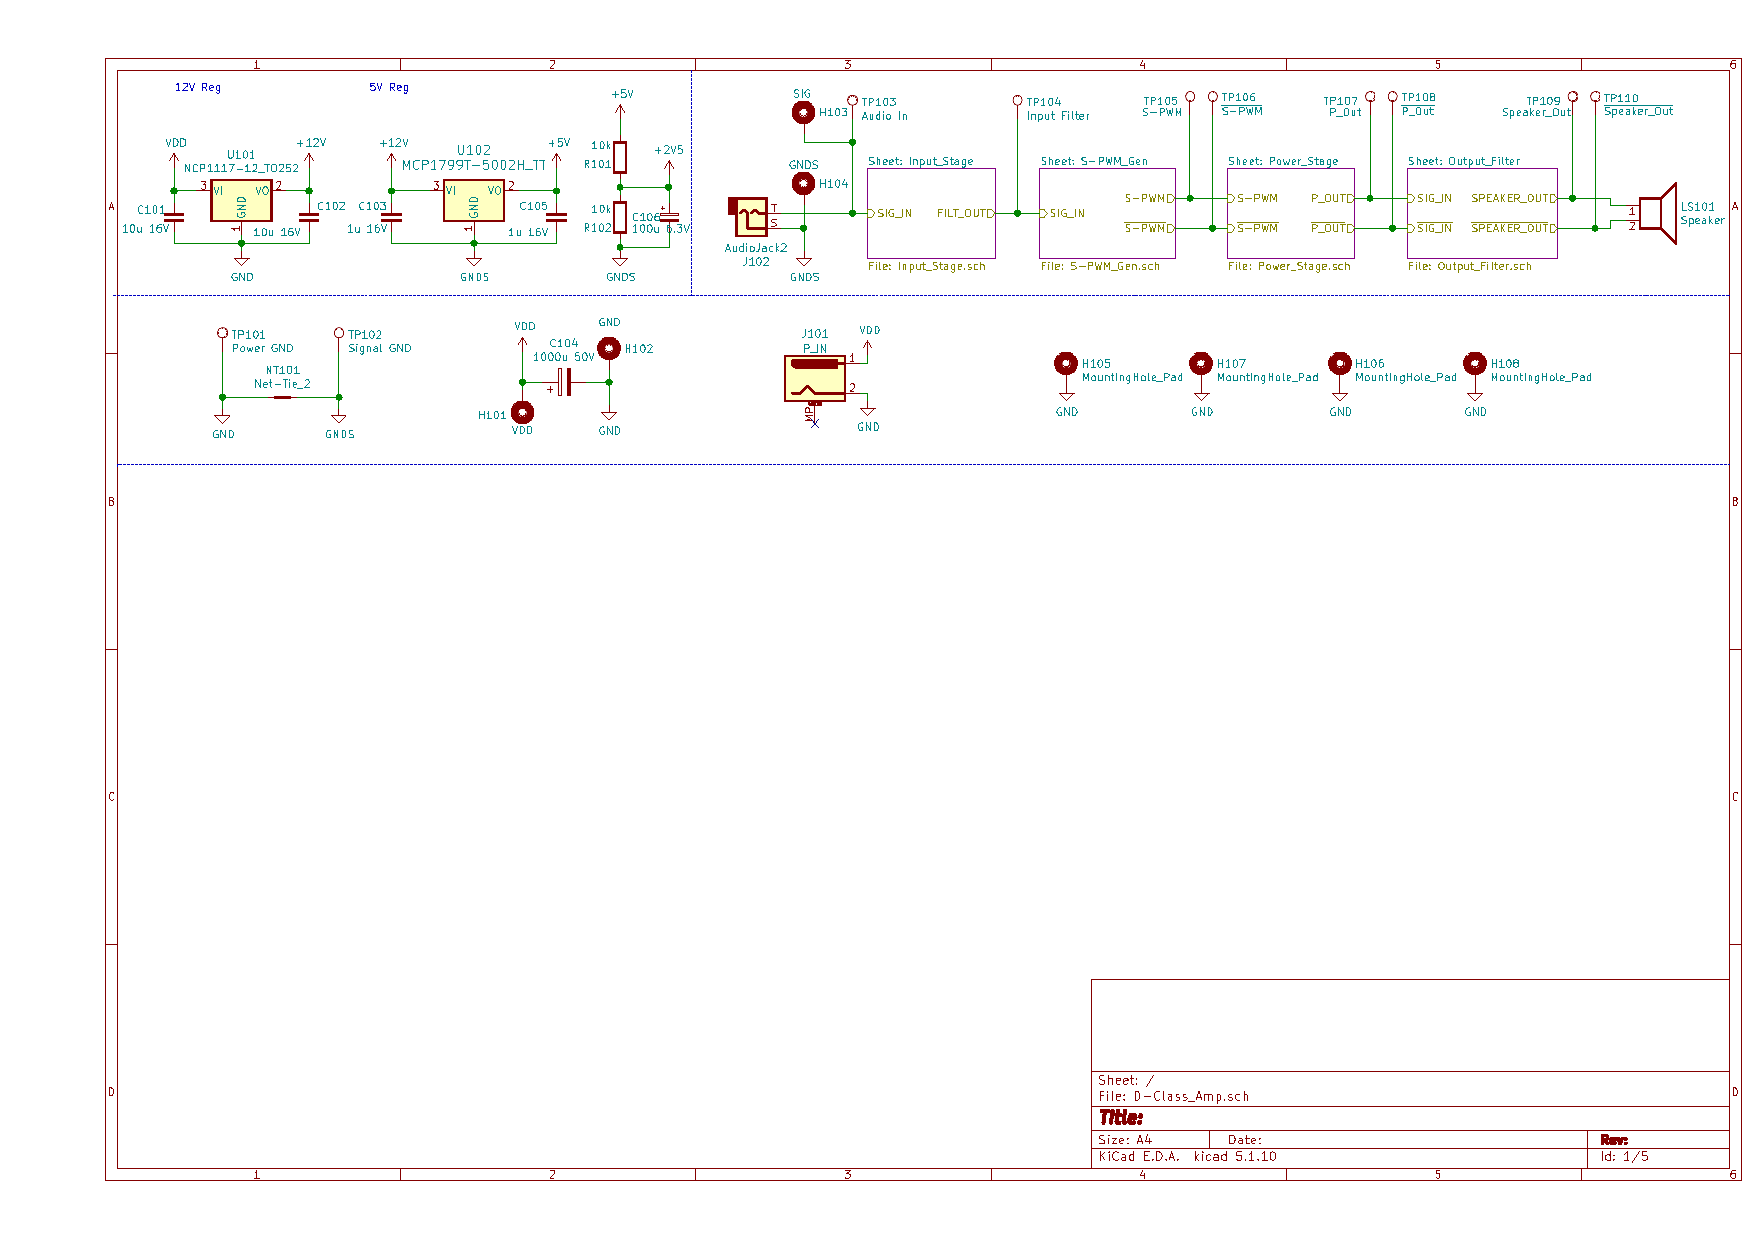
\includegraphics[page=1, trim={18mm 132mm 2mm 10mm},clip,width=0.85\textwidth]{pcb/schematic.pdf}}
    \caption{High level design schematic}
\end{figure}

\subsection{Input Filter}

\begin{figure}[h!]
    \centering
    \frame{\includegraphics[page=2, trim={25mm 70mm 90mm 60mm},clip,width=0.85\textwidth]{pcb/schematic.pdf}}
    \caption{Input filtering schematic}
\end{figure}

\subsection{Audio Sampling \& SPWM}

\begin{figure}[h!]
    \centering
    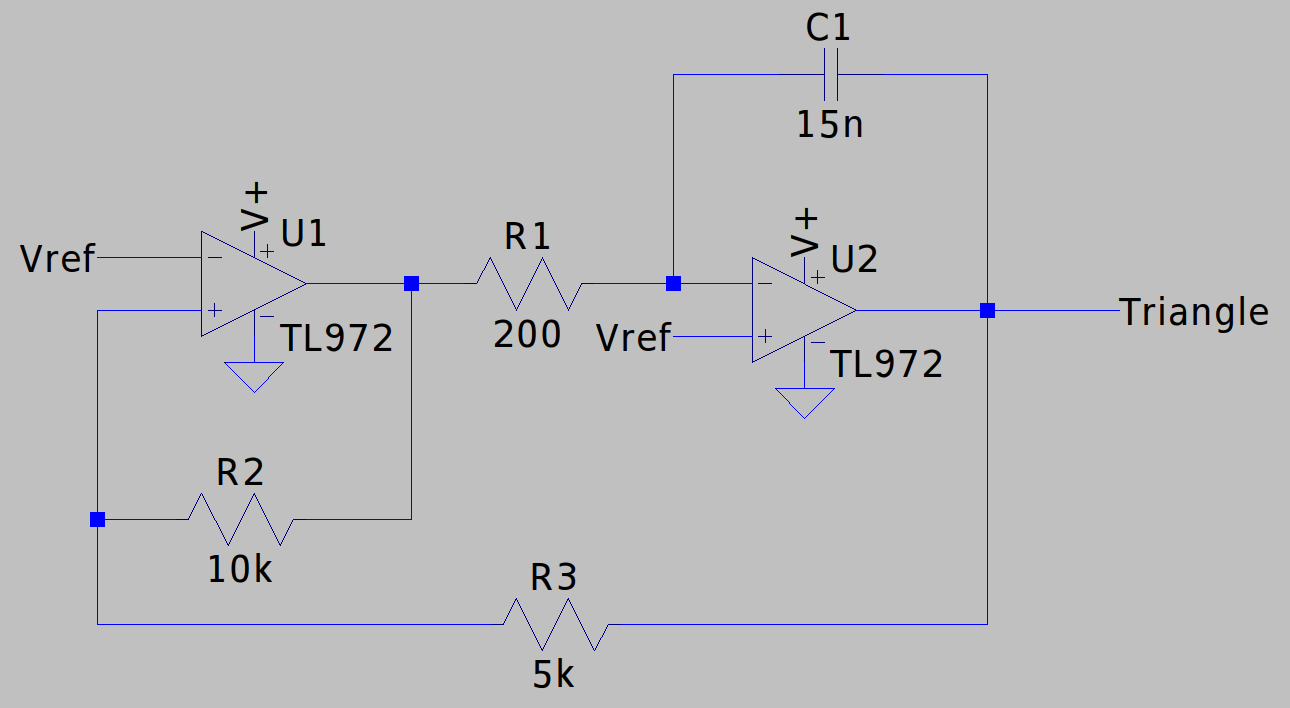
\includegraphics[width=0.6\textwidth]{spwm/circuit.png}
    \caption{Triangle waveform generation citcuit}
\end{figure}

\begin{figure}[h!]
    \centering
    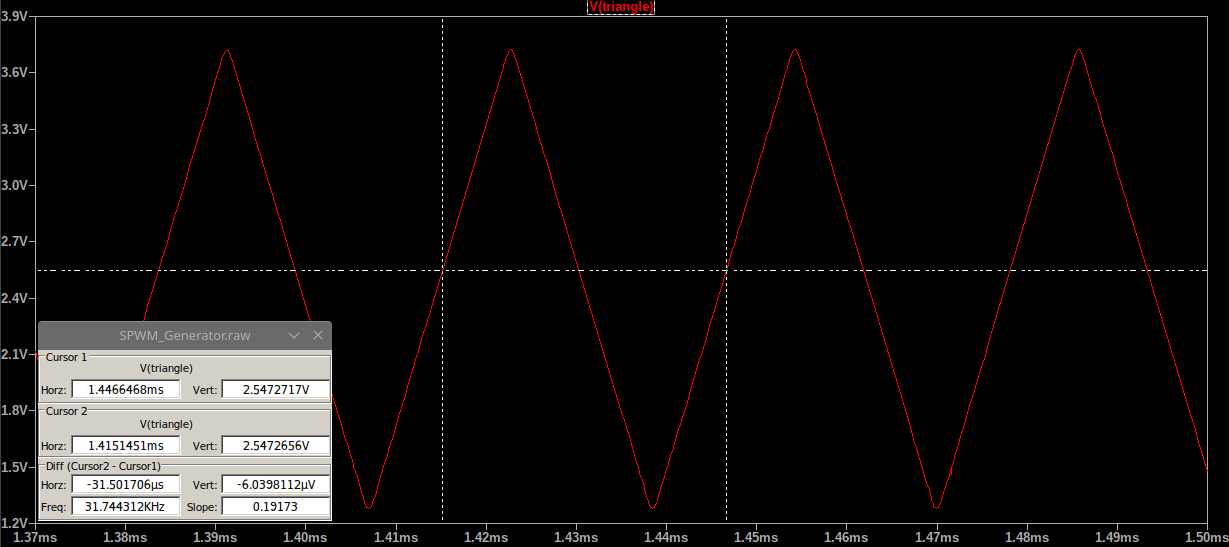
\includegraphics[width=0.8\textwidth]{simulation/triangle_wave.png}
    \caption{Simulation of the generated 32kHz triangle waveform}
\end{figure}


\begin{figure}[h!]
    \centering
    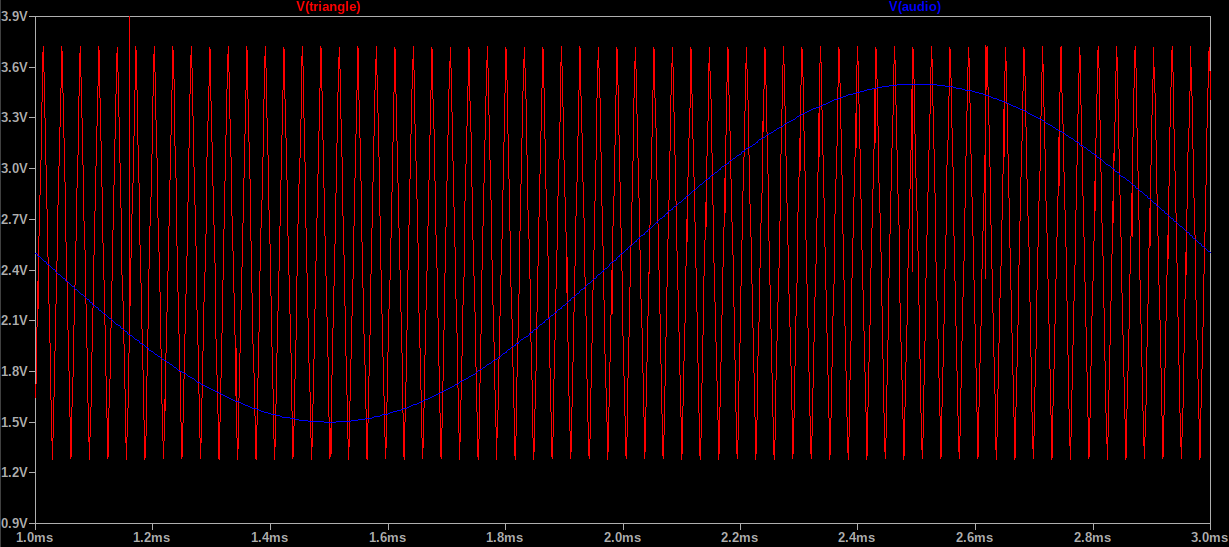
\includegraphics[width=0.8\textwidth]{simulation/sampling.png}
    \caption{Simulation of a 1V peak to peak input signal sampling}
\end{figure}


\begin{figure}[h!]
    \centering
    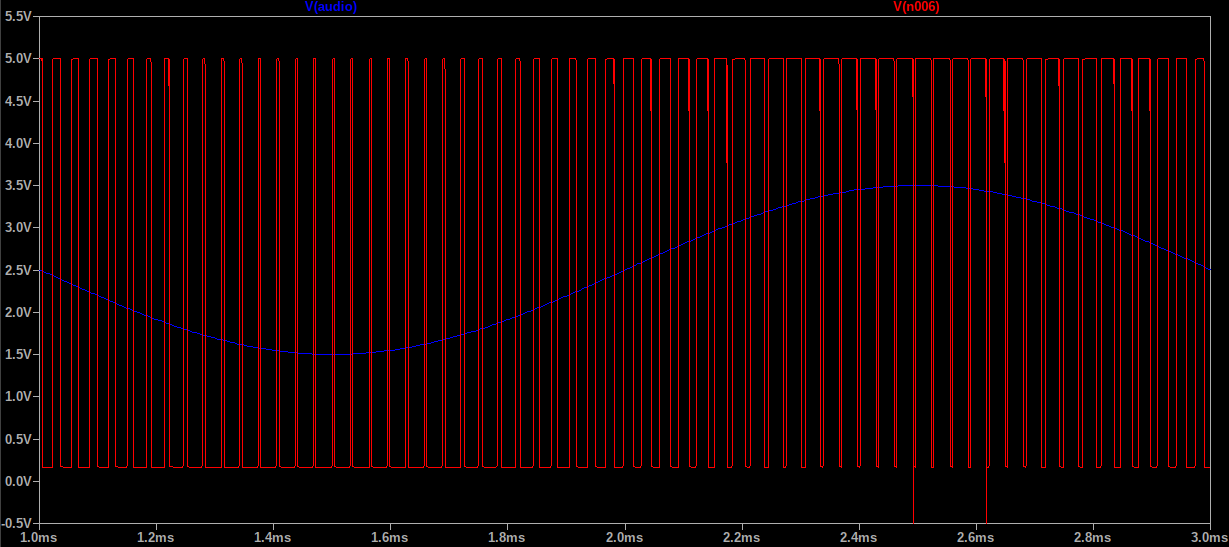
\includegraphics[width=0.8\textwidth]{simulation/spwm_out.png}
    \caption{Simulation of the SPWM comparator output}
\end{figure}

\begin{figure}[h!]
    \centering
    \frame{\includegraphics[page=3, trim={35mm 133.5mm 30mm 15mm},clip,width=0.85\textwidth]{pcb/schematic.pdf}}
    \caption{Sampling triangle wave \& SPWM generation schematic}
\end{figure}

\subsection{Power Stage \& Output Filter}

\begin{figure}[h!]
    \centering
    \frame{\includegraphics[page=5, trim={85mm 149mm 5mm 12mm},clip,width=0.85\textwidth]{pcb/schematic.pdf}}
    \caption{Gate driver schematic}
\end{figure}

\begin{figure}[h!]
    \centering
    \frame{\includegraphics[page=4, trim={115mm 97mm 105mm 75mm},clip,width=0.6\textwidth]{pcb/schematic.pdf}}
    \caption{Output filter schematic}
\end{figure}

\subsection{PCB Design and Layout}


\begin{figure}[h!]
    \centering
    \begin{subfigure}{0.8\textwidth}
        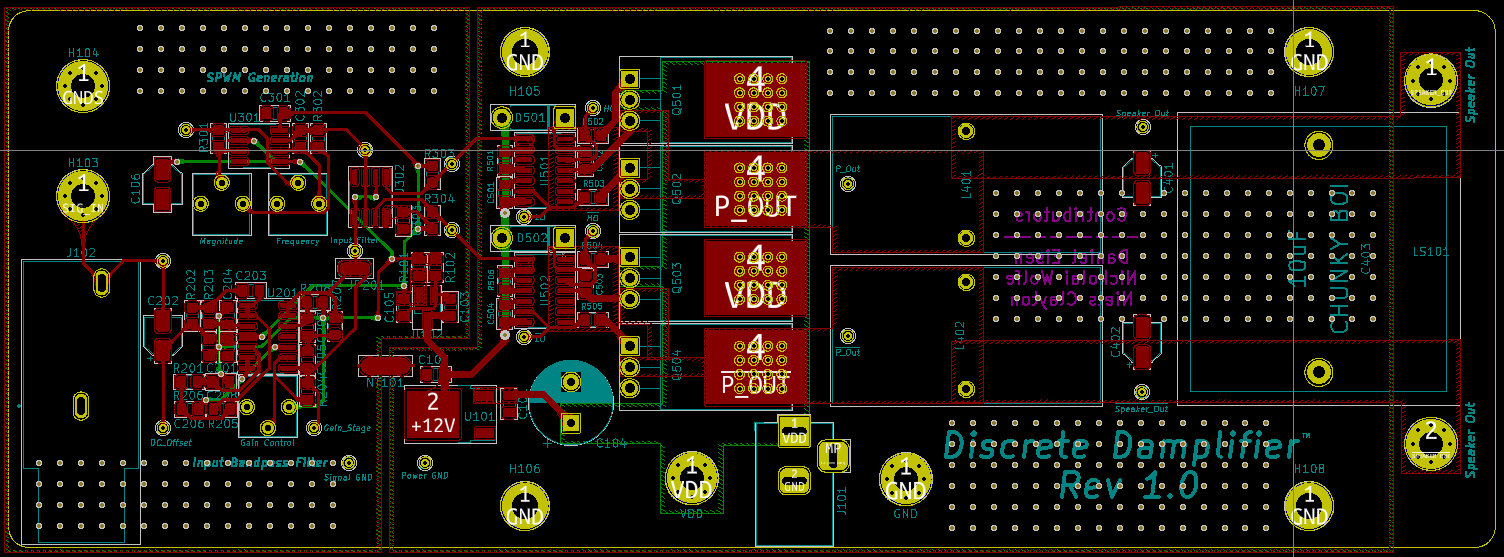
\includegraphics[width=\columnwidth]{pcb/traces.png}
        \subcaption{}
    \end{subfigure}
    \begin{subfigure}{0.8\textwidth}
        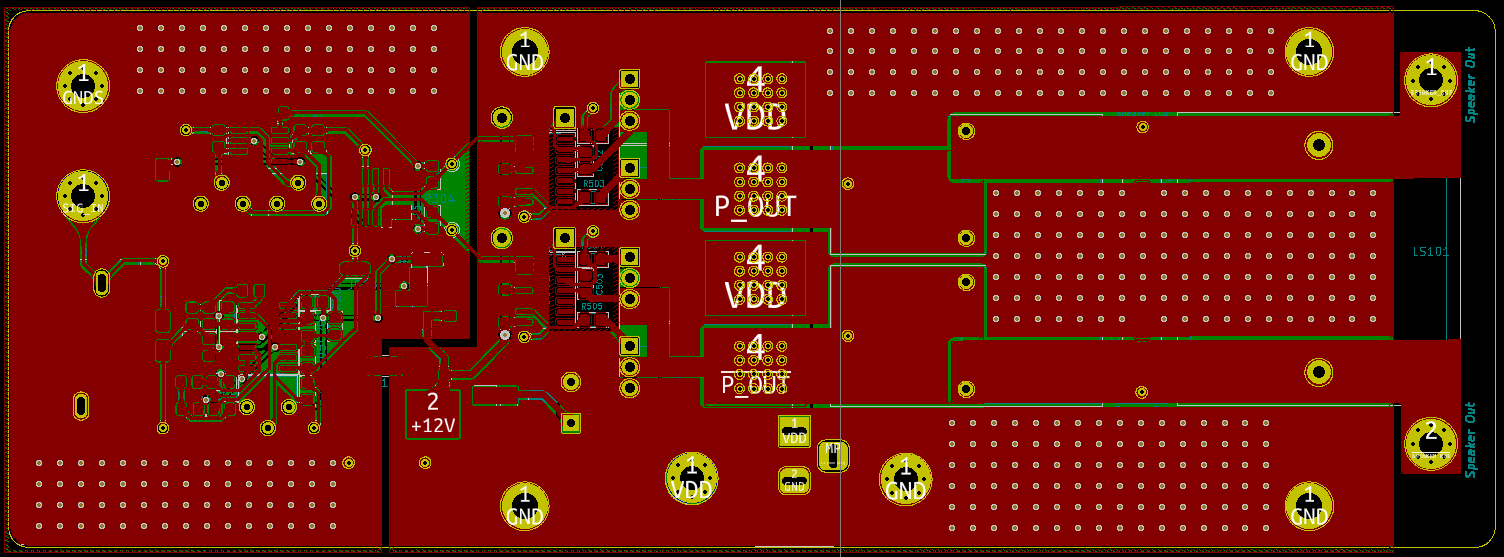
\includegraphics[width=\columnwidth]{pcb/top_layer.png}
        \subcaption{}
    \end{subfigure}
    \begin{subfigure}{0.8\textwidth}
        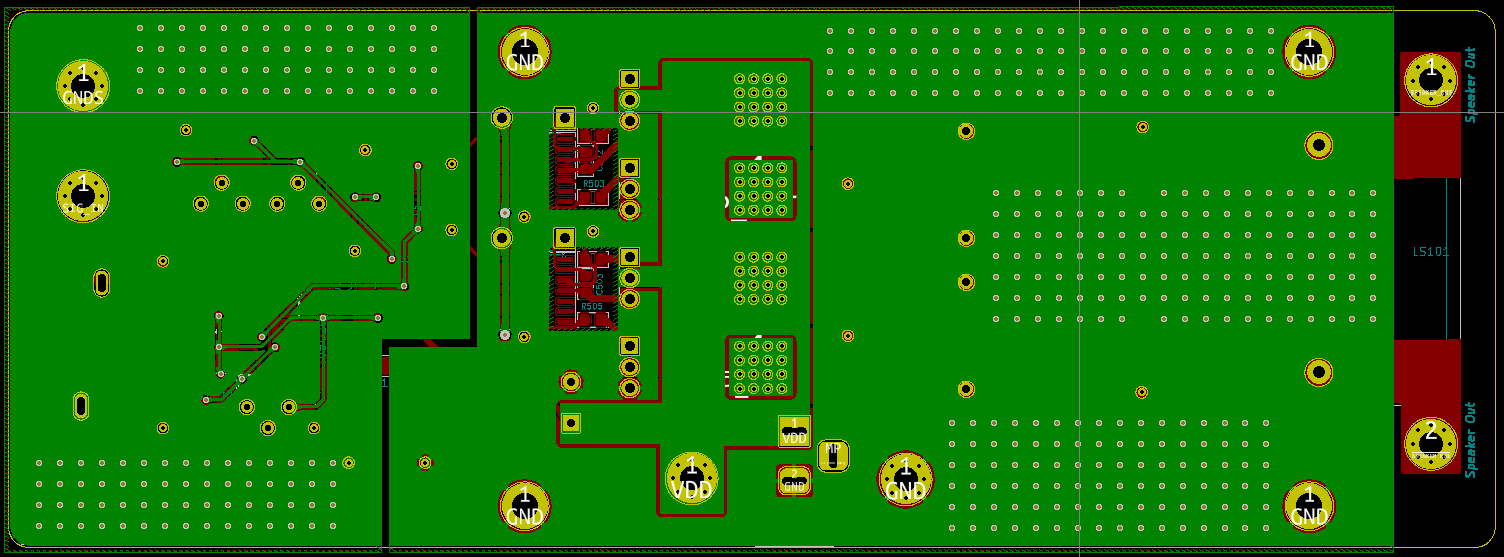
\includegraphics[width=\columnwidth]{pcb/bottom_layer.png}
        \subcaption{}
    \end{subfigure}
    \caption{}
\end{figure}


\section{Implementation}

Here you should discuss the assembly of the amplifier and any problems you faced as a team building the amplifier.

Here, the individual components should also be characterised. For example: if you have a filter, what is the response and how does it compare to the calculated? If you have a triangle wave, how does it look? Is it doing what I should? Why? Why not? How do the inputs/outputs of your comparator look? How does the square wave on the gate of the MOSFETs look?


\begin{figure}[h!]
    \centering
    \begin{subfigure}{0.52\textwidth}
        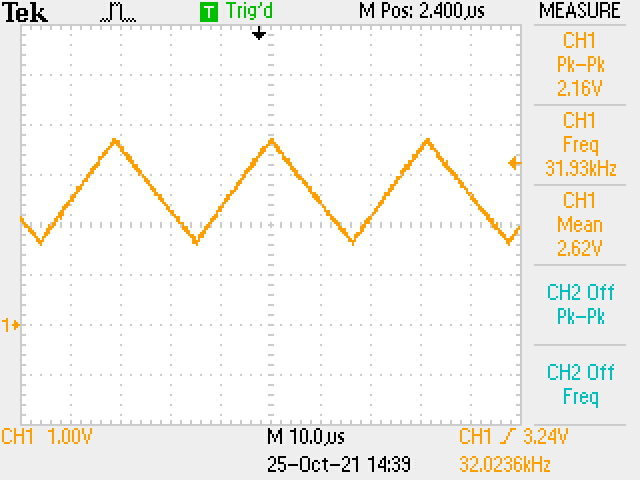
\includegraphics[width=\columnwidth]{spwm/triangle_wave_32kHz.JPG}
        \subcaption{}
    \end{subfigure}
    \begin{subfigure}{0.48\textwidth}
        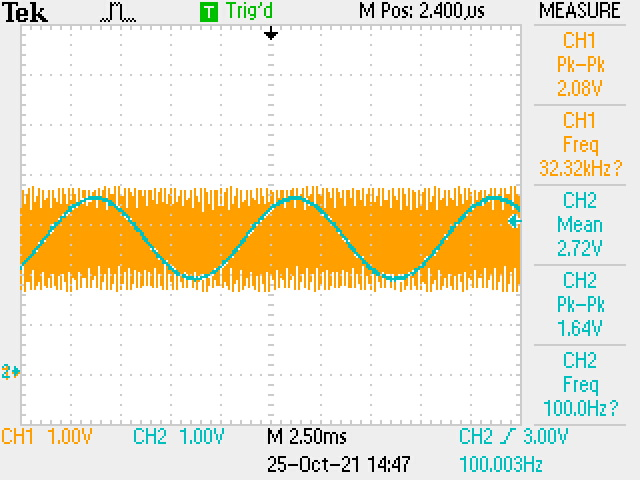
\includegraphics[width=\columnwidth]{spwm/input_sampling_0.JPG}
        \subcaption{}
    \end{subfigure}
    \begin{subfigure}{0.48\textwidth}
        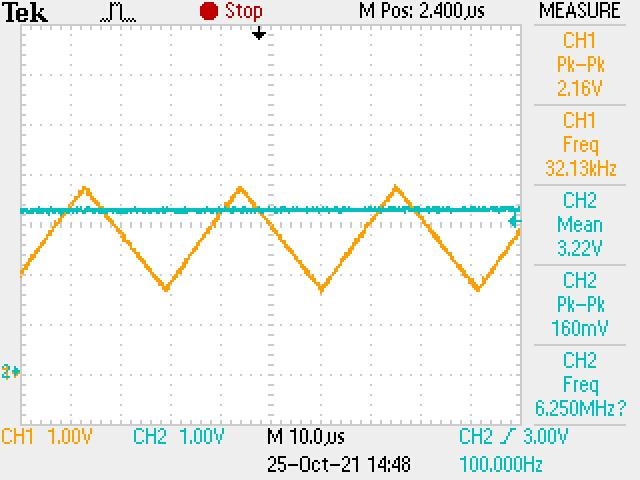
\includegraphics[width=\columnwidth]{spwm/input_sampling_1.JPG}
        \subcaption{}
    \end{subfigure}
    \caption{}
\end{figure}

\begin{figure}[h!]
    \centering
    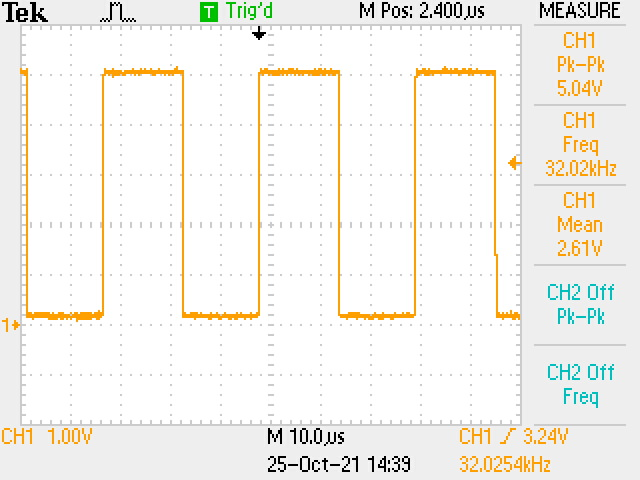
\includegraphics[width=0.65\textwidth]{spwm/spwm_no_input.JPG}
    \caption{Amplifier output bode plot}
\end{figure}


\section{Results}

Here I would expect to see the results of the whole amp, for example: an output wave, analysis of the efficiency, discuss maximum power output (which may be frequency dependent), and THD.


\begin{figure}[h!]
    \centering
    \begin{subfigure}{0.3\textwidth}
        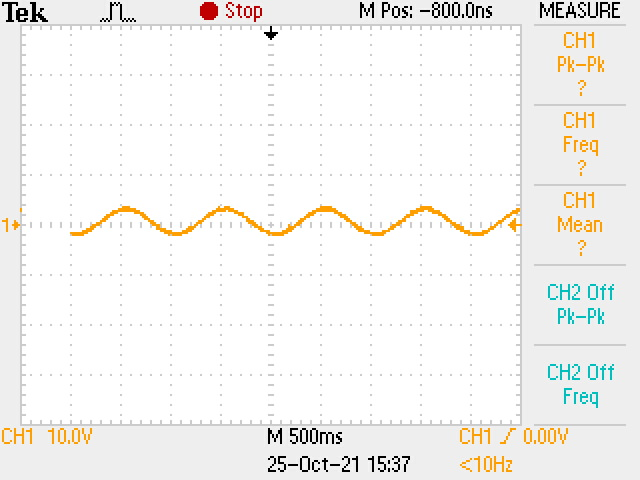
\includegraphics[width=\columnwidth]{power_output/filter_output_1Hz.JPG}
        \subcaption{}
    \end{subfigure}
    \begin{subfigure}{0.3\textwidth}
        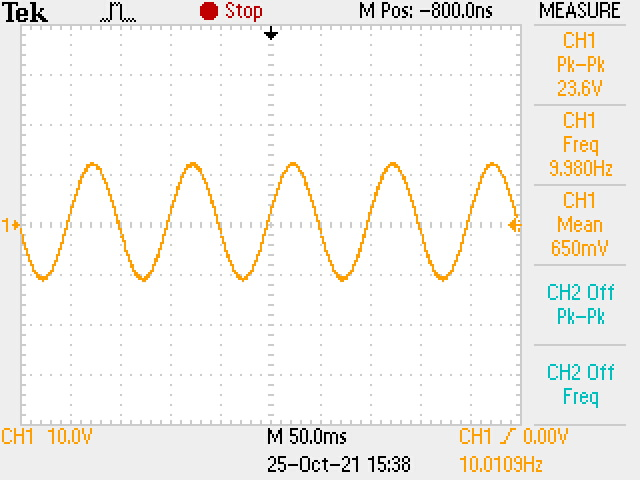
\includegraphics[width=\columnwidth]{power_output/filter_output_10Hz.JPG}
        \subcaption{}
    \end{subfigure}
    \begin{subfigure}{0.3\textwidth}
        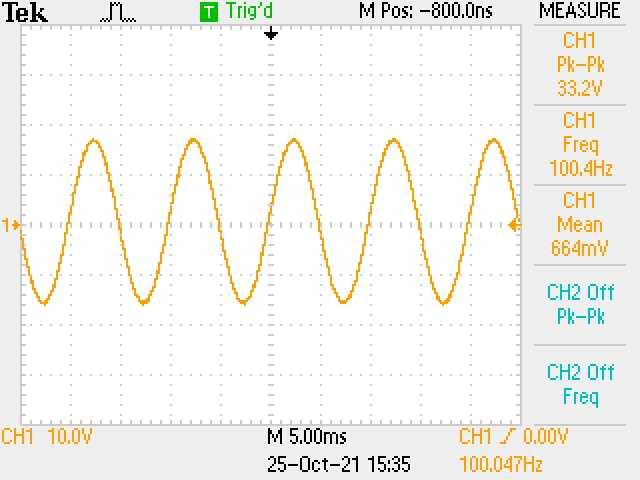
\includegraphics[width=\columnwidth]{power_output/filter_output_100Hz.JPG}
        \subcaption{}
    \end{subfigure}
    \begin{subfigure}{0.3\textwidth}
        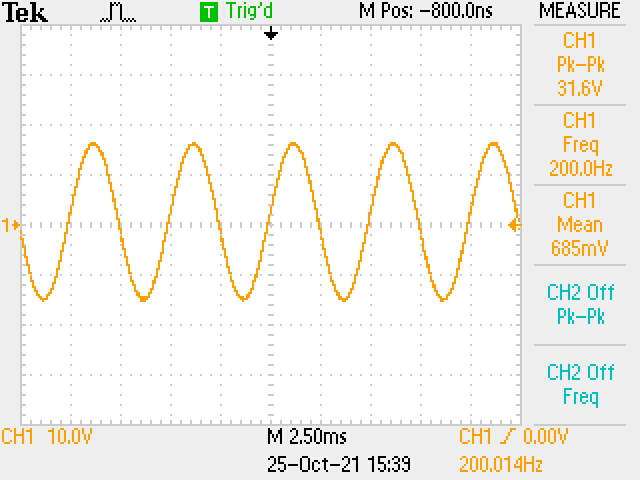
\includegraphics[width=\columnwidth]{power_output/filter_output_200Hz.JPG}
        \subcaption{}
    \end{subfigure}
    \begin{subfigure}{0.3\textwidth}
        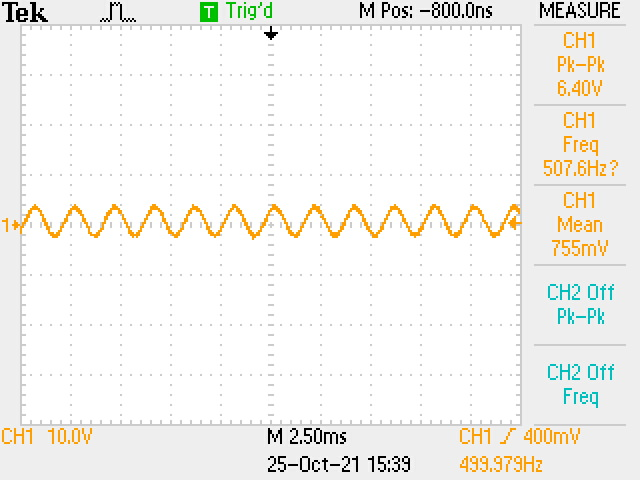
\includegraphics[width=\columnwidth]{power_output/filter_output_500Hz.JPG}
        \subcaption{}
    \end{subfigure}
    \begin{subfigure}{0.3\textwidth}
        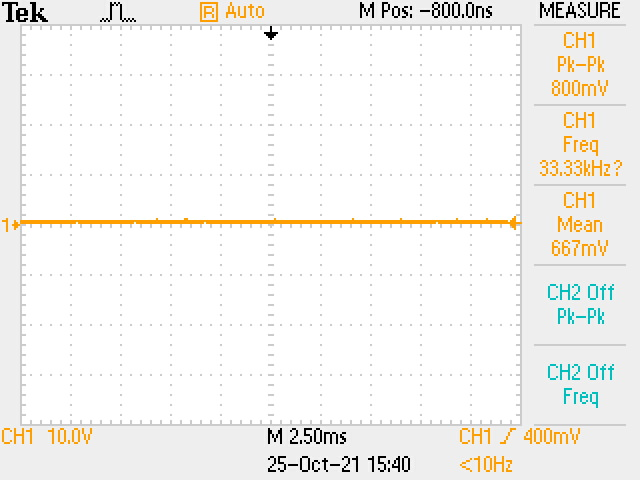
\includegraphics[width=\columnwidth]{power_output/filter_output_2kHz.JPG}
        \subcaption{}
    \end{subfigure}
    \caption{}
\end{figure}


\begin{figure}[h!]
    \centering
    \frame{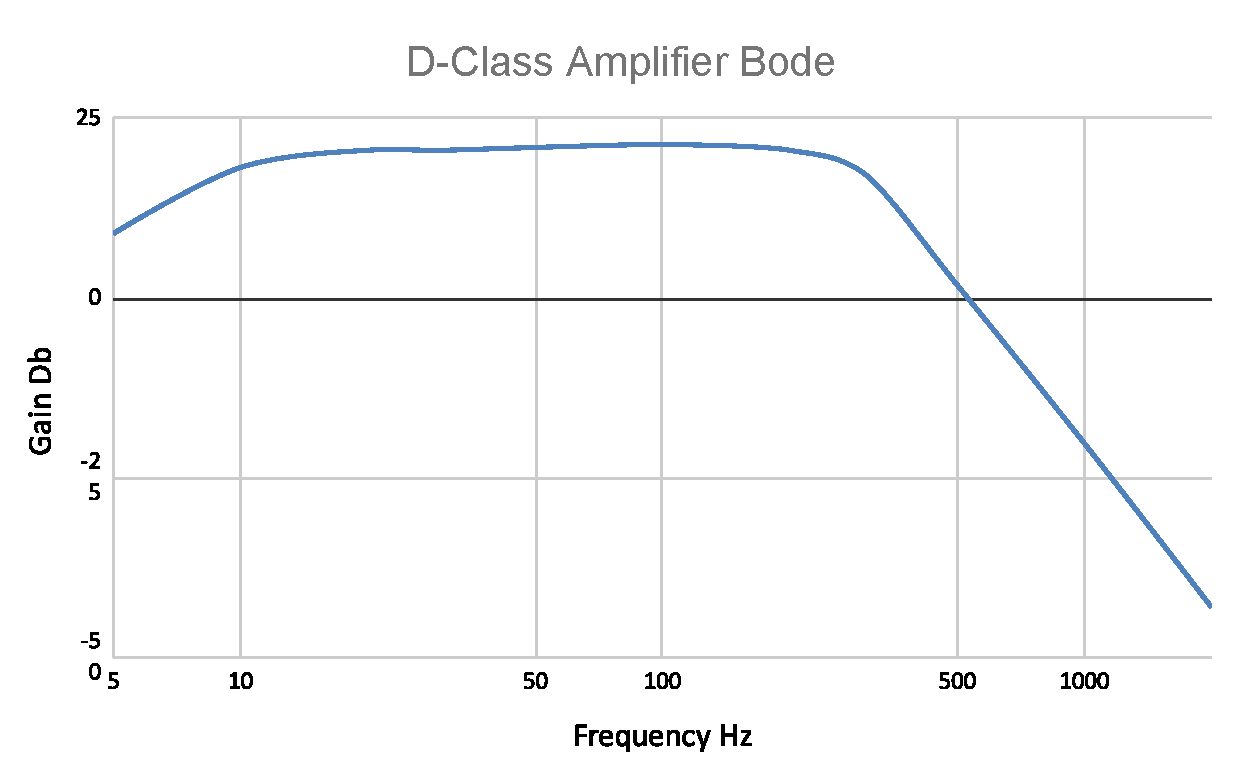
\includegraphics[width=0.85\textwidth]{power_output/amplifier_bode.pdf}}
    \caption{Amplifier output bode plot}
\end{figure}


\begin{figure}[h!]
    \centering
    \frame{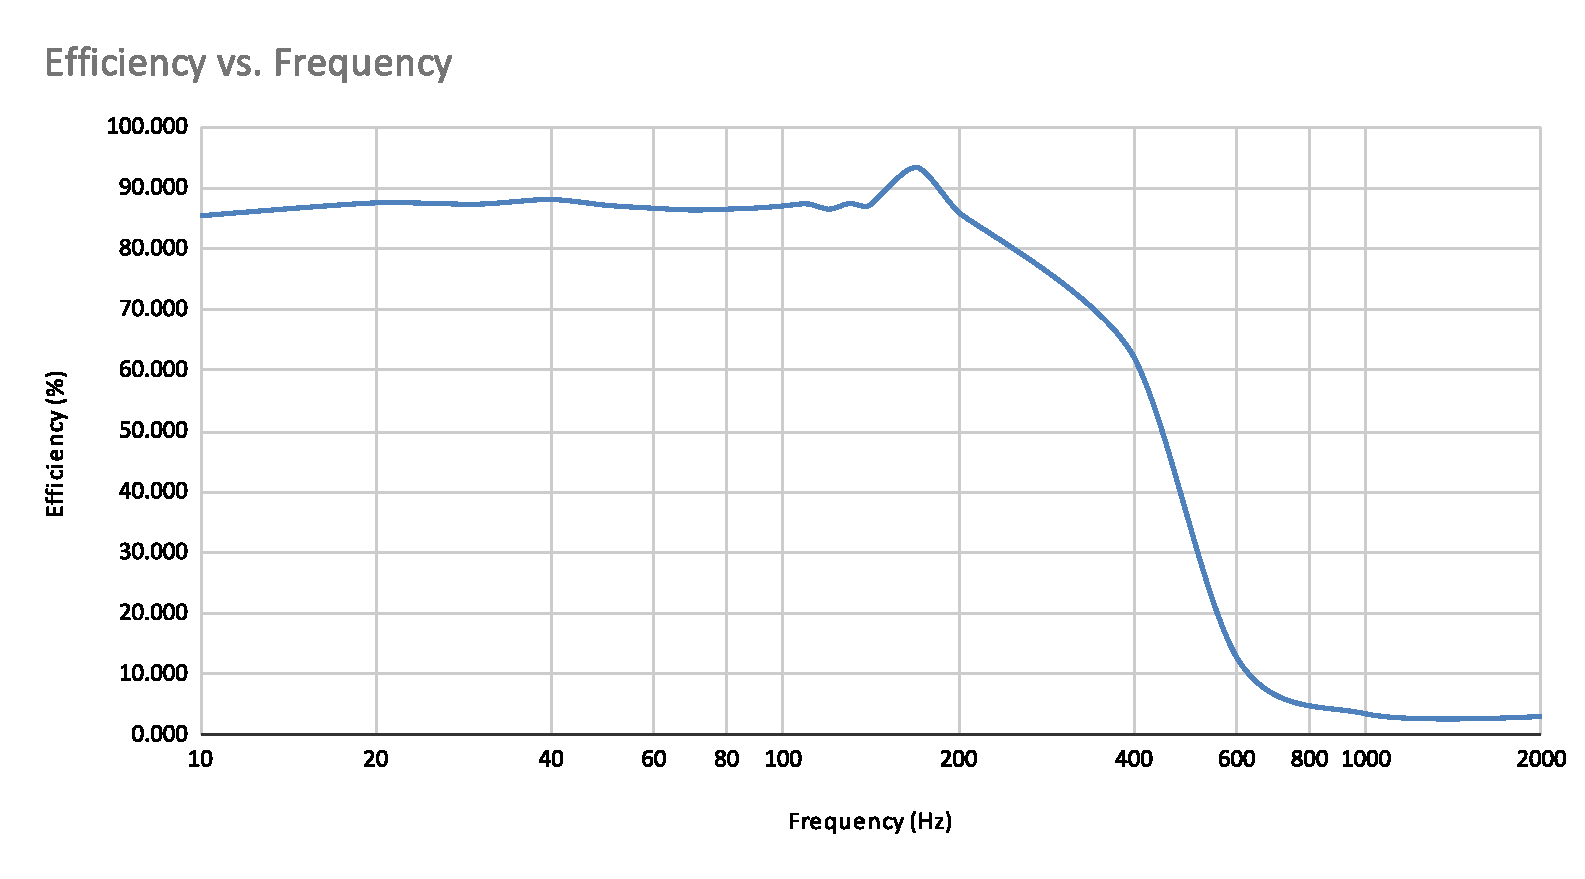
\includegraphics[width=0.85\textwidth]{power_output/Efficiency_vs._Frequency.pdf}}
    \caption{Amplifier output efficiency vs frequency}
\end{figure}


\begin{table}[h!]
    \centering
    \begin{tabular}{l|l}
    \rowcolor[HTML]{E0E0E0} 
    \textbf{Frequency (Hz)} & \textbf{THD (\%)} \\ \hline
    30                 & 1.8               \\
    50                 & 2.2               \\
    100                & 3.2               \\
    200                & 3.3               \\
    300                & 3.5               \\
    500                & 3.2              
    \end{tabular}
    \caption{Output total harmonic distortion across frequency}
    \label{T:THD}
\end{table}

\section{Conclusions}

What worked, didn’t work? How would you change your approach? Any interesting insights?

\clearpage
\section*{Appendix}
\subsection*{Input Filter}
\begin{figure}[h!]
  \centering
  \begin{subfigure}{0.3\textwidth}
    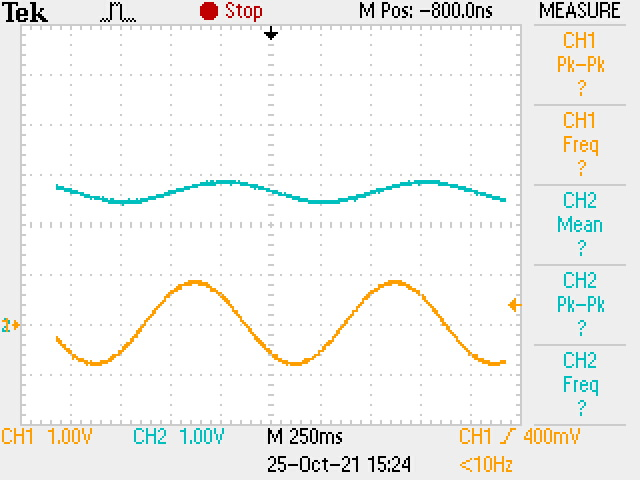
\includegraphics[width=\columnwidth]{input_filter/input_1Hz.JPG}
    \subcaption{1Hz}
  \end{subfigure}
  \begin{subfigure}{0.3\textwidth}
    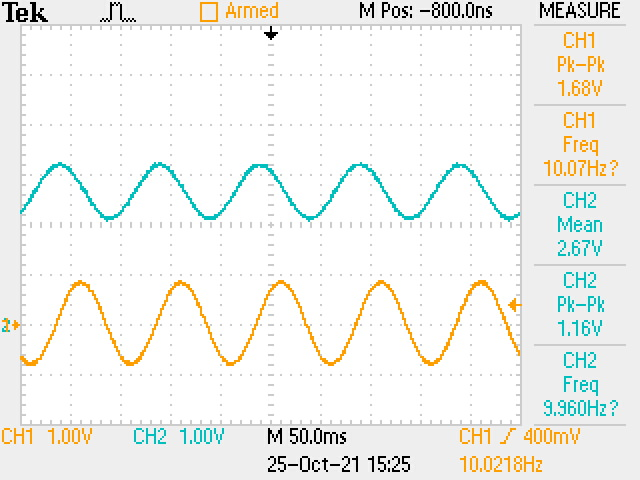
\includegraphics[width=\columnwidth]{input_filter/input_10Hz.JPG}
    \subcaption{10Hz}
  \end{subfigure}
  \begin{subfigure}{0.3\textwidth}
    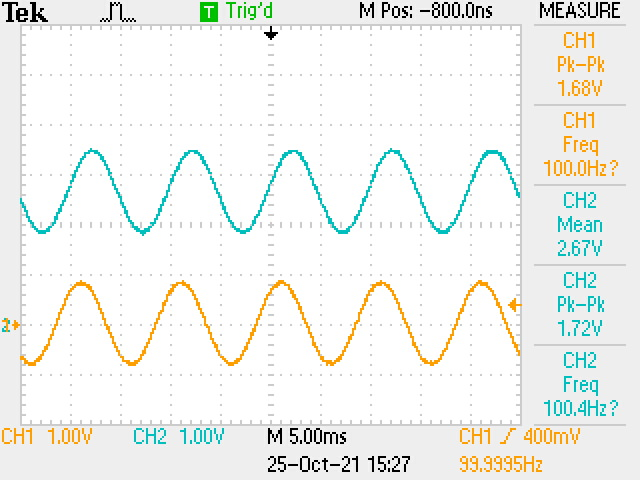
\includegraphics[width=\columnwidth]{input_filter/input_100Hz.JPG}
    \subcaption{100Hz}
  \end{subfigure}
  \begin{subfigure}{0.3\textwidth}
    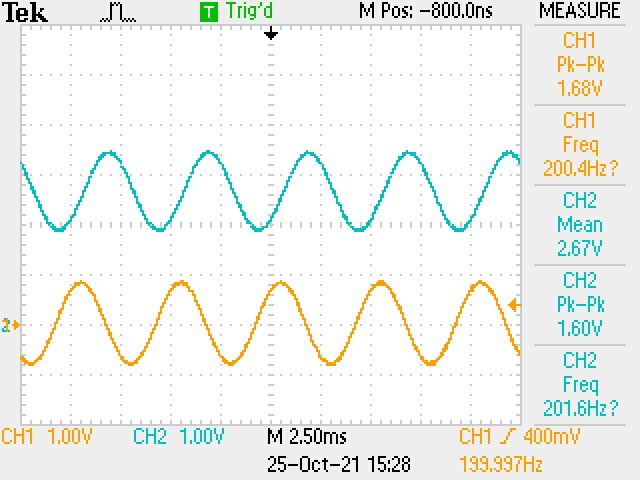
\includegraphics[width=\columnwidth]{input_filter/input_200Hz.JPG}
    \subcaption{200Hz}
  \end{subfigure}
  \begin{subfigure}{0.3\textwidth}
    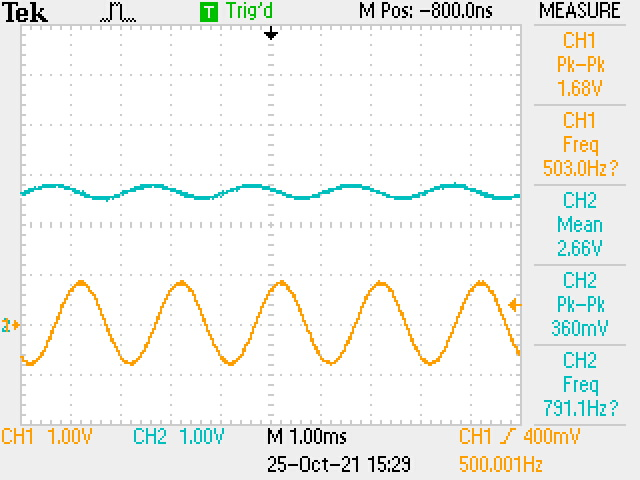
\includegraphics[width=\columnwidth]{input_filter/input_500Hz.JPG}
    \subcaption{500Hz}
  \end{subfigure}
  \begin{subfigure}{0.3\textwidth}
    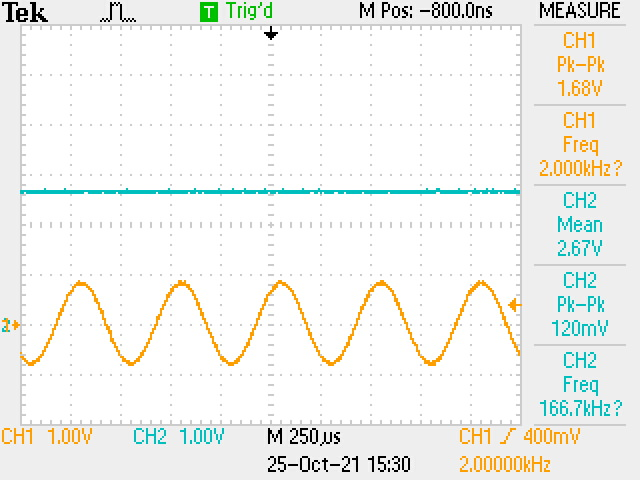
\includegraphics[width=\columnwidth]{input_filter/input_2kHz.JPG}
    \subcaption{2kHz}
  \end{subfigure}
  \caption{Input filter operation across frequencies, input signal (yellow) vs filter output (blue)}
\end{figure}


\end{document}